\documentclass[conference]{IEEEtran}
\usepackage{graphicx}

\begin{document}

\title{The proposal for revealing unusual events in GitHub repositories}


\author{\IEEEauthorblockN{Xiyu Zhang}
\IEEEauthorblockA{a1673016\\School of Computer Science\\
The University of Adelaide\\
Adelaide, Australia\\
Email: \\a1673016@student.adelaide.edu.au}
\and
\IEEEauthorblockN{Jiexin Li}
\IEEEauthorblockA{a1714727\\School of Computer Science\\
The University of Adelaide\\
Adelaide, Australia\\
Email: \\a1714727@student.adelaide.edu.au}
\and
\IEEEauthorblockN{Tianshuo Zhang}
\IEEEauthorblockA{a1711997\\School of Computer Science\\
The University of Adelaide\\
Adelaide, Australia\\
Email: \\a1711997@student.adelaide.edu.au}}


\maketitle


\begin{abstract}

At present, current large scale projects need developers to pay more attention on considering its details. Furthermore, establishing a project to implement an useful tool that can be able to assist developers to know what has happened in their projects, that is needed. Moreover, this project is based on previous researches by Christoph et al. Its purpose is to implement a tool which can be able to detect unusual events in GitHub repositories. After that, showing results to developers in order to remind them what unusual events have existed in their repositories. During the whole process, we will cooperate with some mathematical students in order to try to define new types of unusual events. Moreover, we have listed deliverables and its details, also illustrating the Gantt chart and individual contributions for milestones.
\end{abstract}



%%%%%%%%%%%%%%%%%%%%%%%%%%%%%%%%%%%%%%%%%%%%%%%%%%%%%%%%%%%%%%%%%%%%%%%%%%%%%%%%
\section{INTRODUCTION}

At present, a large amount of data is updated and uploaded every day in GitHub.As each project grows, developers need to think more and more about the details of the project. This makes it possible for developers to take into account some of the details of the project. And this can lead to a whole project's vulnerability even paralyze the project.\\

Christoph et al. carried out data extraction and induction for 200 projects and 14 developers from GitHub on this issue. And through these data, the 6 operations were defined and named as unusual events and propose a reliable solution. For instance, adding multiple lines of code in a short period of time may lead to the emergence of bug. They believe that marking out unusual events can help developers better understand the progress of their own projects. In addition, it also helps them to take care of the easily overlooked details of the project.At the end of the Christoph et al paper, they suggest that they need to have a software to implement their ideas. We will implement this software and define more types of unusual events with them.

\section{Motivation}

In the process of modern software development, with the progress of the project, more and more details need to be paid attention to. This is not perfect for developers. This is likely to lead to obstacles to development. The purpose of this project is to reduce the occurrence of such a situation. First, define some unusual events that may be neglected. When these events happen, remind developers to improve the quality of projects. 

\subsection{Novelty Statement}

In the course of the project, we will do the statistics and analysis of the data with some mathematical students. Through experiments and studies to define new types of unusual events that are likely to be ignored.


\section{Background and Related work}

Nowadays, GitHub is the most famous code repository in the world, million, even billion, lines of code are stored in there. It is a Git repository based on web hosting service, and it can control all the distributed revision and manage source code. However, if you got a difficult issue which will take a long time to solve, many unusual comments will be attracted by some controversial pull requests, and adding and deleting files may happen because of disruptive commits.\\

Therefore, the commits, issues or pull requests cannot be possibly known immediately when the developer participates in a large software project. Nevertheless, there is no need to know all details which happen in the code. There are some high-level tools to attract developers’ attention for any activities in the code, for example Crystal or WeCode. However, those tools provide limited information for the project.\\

Christoph et al.’s paper has defined some unusual events, for instance, an unusual commit message or uploading a lot of files. They presented 140 users from 200 projects in Github. Finally, the very useful information is deleting, adding, modifying for the developers; meanwhile, the comments on issues and pull requests are also useful for them [2]. 


\section{Studied subjects / datasets}

The previous stage of our project may use the examples and data from the paper “Unusual Events in GitHub Repositories” written by Christoph et al. This paper has defined the unusual events to some extent. For the next step, we will collect data from other GitHub repositories as test sample, such as twbs/bootrap in GitHub. Firstly, we can detect consistently this repository as our original datasets because it big enough and many commits, pull requests, issues in it. In short, the first datasets we will get is from other repositories. At the later stage of this project, the datasets should be all the projects in GitHub.\\

At the same time, we will continuously define the unusual events for the next datasets. The next datasets will be the filtered datasets. This means that we will filter the original data from repositories by defined unusual events. Unfortunately, how to define an unusual event is difficult. The specific method to define unusual events should be discussed someone work or study in mathematics department. They will explain and build a formula for our project to define the unusual events, so that we can program the filter to wash the original datasets.


\section{Details of Expected Deliverables}

The ultimate goal of this project is to complete a system that has the functions of:
\bigskip
\begin{itemize}
\item Find out the unusual events in the GitHub project;

\item Can be reviewed in the results list of different events;
\item Dynamic updates are displayed for the results of unusual events.
\end{itemize}
\bigskip
Temporarily, for the implementation of these functions, we have a few current deliverable plans:\\

\paragraph{\textbf{Milestone 1}}
There are no deliverables in this state due to the fact that we were doing some preparation works in the beginning.\\

\paragraph{\textbf{Milestone 2}}
A basic system was completed fourth weeks ago. The system can connect to the local database and screen for a basic unusual event. For example, find a project from GitHub or local database, and than pick up the code where the number of comments more than five.\\

\paragraph{\textbf{Milestone 3}}
The connection to GitHub was completed seventh weeks ago, and the unusual events we had been screened for.\\

\paragraph{\textbf{Milestone 4}}
Complete the screening of all the unusual events that have been defined tenth weeks ago.\\


\section{The Gantt Chart}

Since the first lecture of Software Engineering Project Part A at week 1, we have never stop to work on that. After the first lecture, all teammates decided the topic that “Revealing unusual events in GitHub repositories“. After that, we have read some related publications which is from our supervisor. Moreover, we analyzed some requirements for this project and confirmed that with our supervisor. And than, we started to design the front and back ends, also doing some practices with useful recommended tools (Such as Bootstrap, SparkJava and HeroKu etc.) in order to be more efficient in this project. In the process of development, we decided to implement the most basic functions. After discussion with supervisor, we are going to spend a few time to build the running environment of recommended tools in the beginning of development. Further, implementing the following functions step by step, such as the front and back-end, login with GitHub account, detecting and showing unusual events etc. Lastly, we will use couple days to do testing before the due date of each milestone. The Gantt chart of the above process as Figure 1:


\begin{figure}[!ht]
\centering
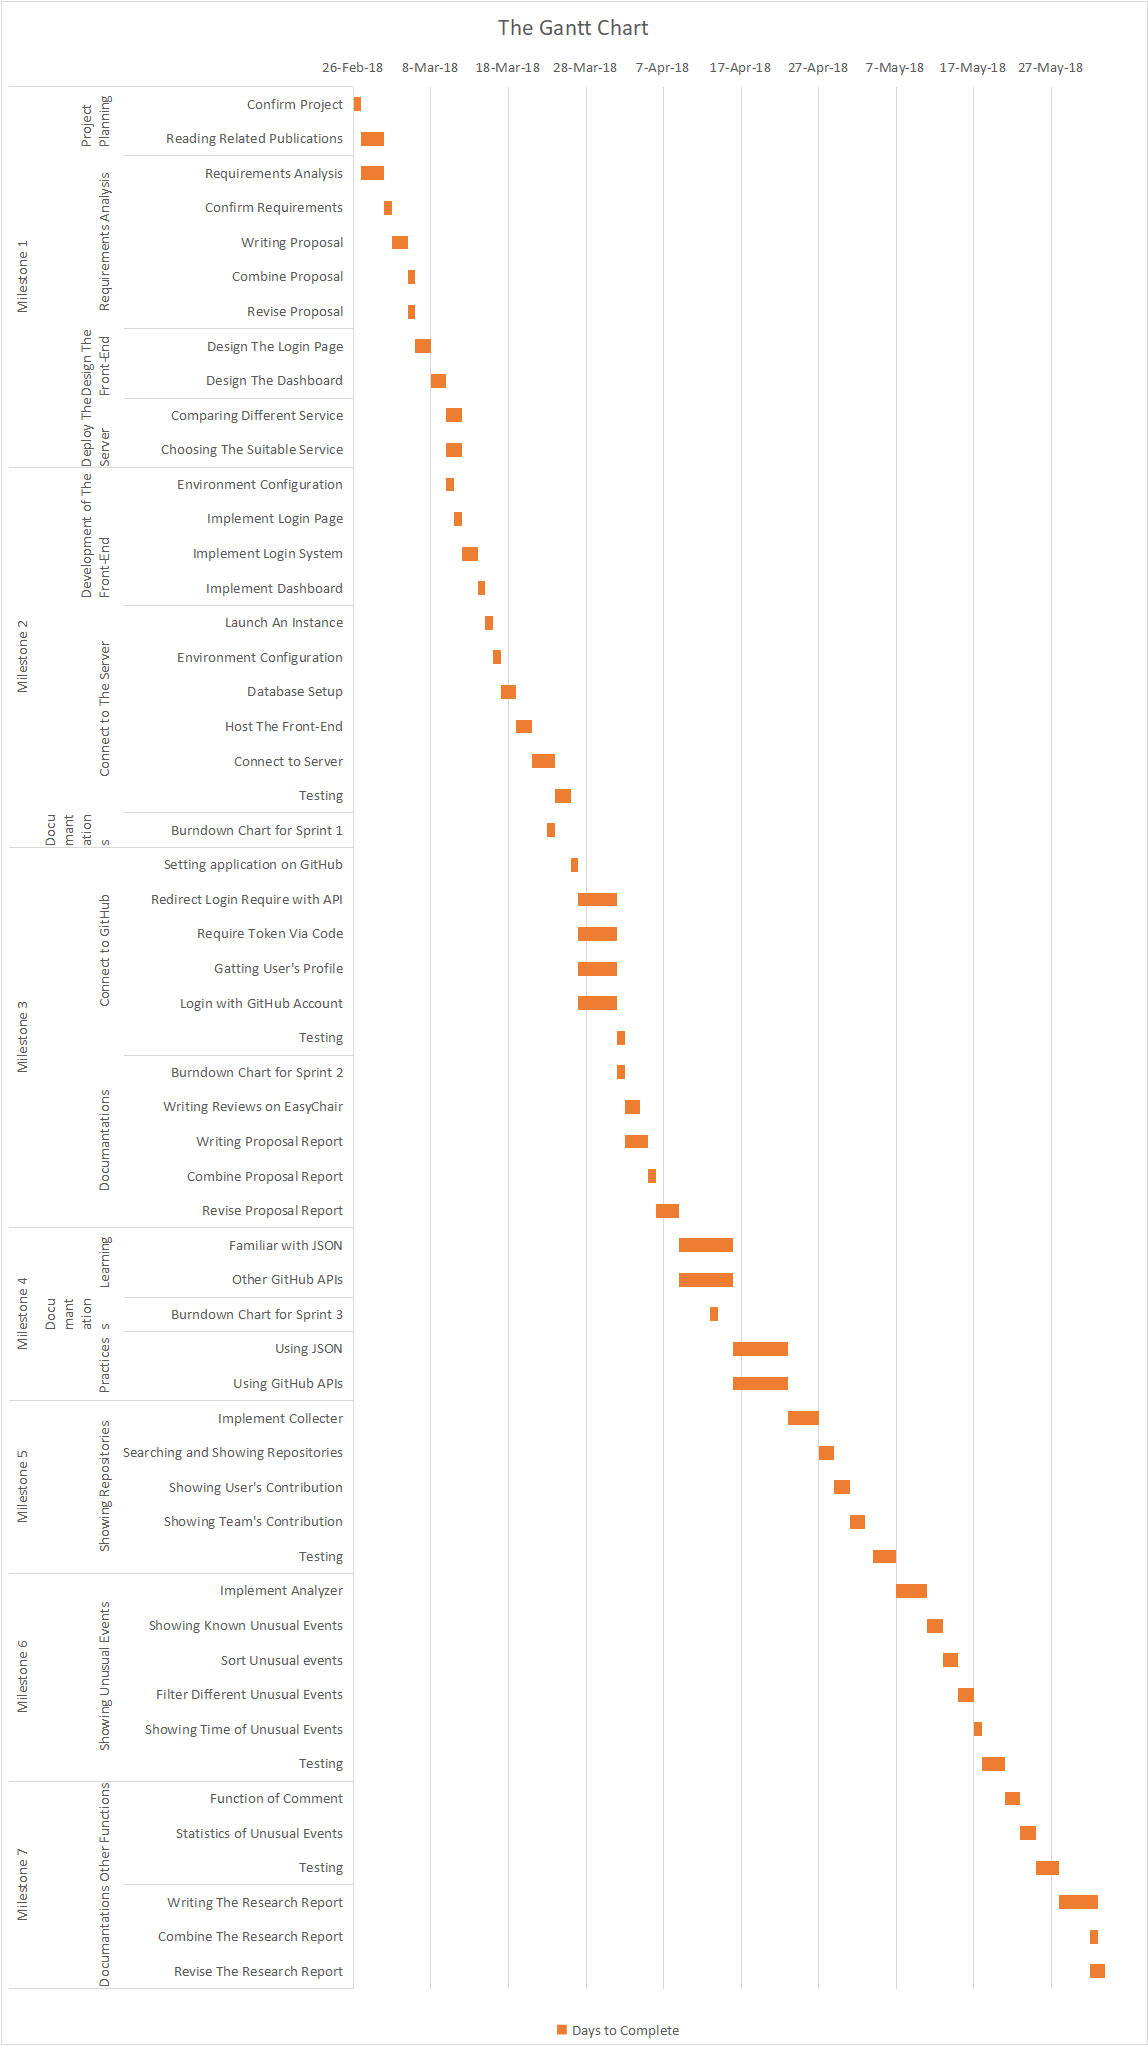
\includegraphics[scale=0.35]{The_Gantt_Chart}
\caption{The Gantt chart for this project}
\end{figure}


\section{Individual Contributions}


\paragraph{\textbf{Xiyu Zhang (Responsibility: The back-end)}}
\medskip
\begin{itemize}
\item Design and Implement the back-end
\item Combining documents
\end{itemize}
\bigskip

\paragraph{\textbf{Jiein Li (Responsibility: The front-end)}}
\medskip
\begin{itemize}
\item Design and Implement the front-end
\item Produce quality management
\end{itemize}
\bigskip

\paragraph{\textbf{Tianshuo Zhang (Responsibility: The back-end)}}
\medskip
\begin{itemize}
\item Connecting the GitHub API with the front-end
\item Testing to the prototype
\end{itemize}


\begin{thebibliography}{99}

\bibitem{c1} Treude C, Figueira Filho F, Kulesza U. Summarizing and measuring development activity[C]//Proceedings of the 2015 10th Joint Meeting on Foundations of Software Engineering. ACM, 2015: 625-636.\\

\bibitem{c2} Treude C, Leite L, Aniche M. Unusual Events in GitHub Repositories[J]. arXiv preprint arXiv:1710.01943, 2017.\\

\bibitem{c3} Leite L, Treude C, Figueira Filho F. UEDashboard: awareness of unusual events in commit histories[C]//Proceedings of the 2015 10th Joint Meeting on Foundations of Software Engineering. ACM, 2015: 978-981.\\


\end{thebibliography}


\end{document}